% Options for packages loaded elsewhere
% Options for packages loaded elsewhere
\PassOptionsToPackage{unicode}{hyperref}
\PassOptionsToPackage{hyphens}{url}
%


\PassOptionsToPackage{table}{xcolor}

\documentclass[
  11pt,
  letterpaper,
]{article}
\usepackage{xcolor}
\usepackage[margin = 0.75in]{geometry}
\usepackage{amsmath,amssymb}
\setcounter{secnumdepth}{5}
\usepackage{iftex}
\ifPDFTeX
  \usepackage[T1]{fontenc}
  \usepackage[utf8]{inputenc}
  \usepackage{textcomp} % provide euro and other symbols
\else % if luatex or xetex
  \usepackage{unicode-math} % this also loads fontspec
  \defaultfontfeatures{Scale=MatchLowercase}
  \defaultfontfeatures[\rmfamily]{Ligatures=TeX,Scale=1}
\fi
\usepackage{lmodern}
\ifPDFTeX\else
  % xetex/luatex font selection
\fi
% Use upquote if available, for straight quotes in verbatim environments
\IfFileExists{upquote.sty}{\usepackage{upquote}}{}
\IfFileExists{microtype.sty}{% use microtype if available
  \usepackage[]{microtype}
  \UseMicrotypeSet[protrusion]{basicmath} % disable protrusion for tt fonts
}{}
\usepackage{setspace}
\makeatletter
\@ifundefined{KOMAClassName}{% if non-KOMA class
  \IfFileExists{parskip.sty}{%
    \usepackage{parskip}
  }{% else
    \setlength{\parindent}{0pt}
    \setlength{\parskip}{6pt plus 2pt minus 1pt}}
}{% if KOMA class
  \KOMAoptions{parskip=half}}
\makeatother


\usepackage{longtable,booktabs,array}
\usepackage{calc} % for calculating minipage widths
% Correct order of tables after \paragraph or \subparagraph
\usepackage{etoolbox}
\makeatletter
\patchcmd\longtable{\par}{\if@noskipsec\mbox{}\fi\par}{}{}
\makeatother
% Allow footnotes in longtable head/foot
\IfFileExists{footnotehyper.sty}{\usepackage{footnotehyper}}{\usepackage{footnote}}
\makesavenoteenv{longtable}
\usepackage{graphicx}
\makeatletter
\newsavebox\pandoc@box
\newcommand*\pandocbounded[1]{% scales image to fit in text height/width
  \sbox\pandoc@box{#1}%
  \Gscale@div\@tempa{\textheight}{\dimexpr\ht\pandoc@box+\dp\pandoc@box\relax}%
  \Gscale@div\@tempb{\linewidth}{\wd\pandoc@box}%
  \ifdim\@tempb\p@<\@tempa\p@\let\@tempa\@tempb\fi% select the smaller of both
  \ifdim\@tempa\p@<\p@\scalebox{\@tempa}{\usebox\pandoc@box}%
  \else\usebox{\pandoc@box}%
  \fi%
}
% Set default figure placement to htbp
\def\fps@figure{htbp}
\makeatother


% definitions for citeproc citations
\NewDocumentCommand\citeproctext{}{}
\NewDocumentCommand\citeproc{mm}{%
  \begingroup\def\citeproctext{#2}\cite{#1}\endgroup}
\makeatletter
 % allow citations to break across lines
 \let\@cite@ofmt\@firstofone
 % avoid brackets around text for \cite:
 \def\@biblabel#1{}
 \def\@cite#1#2{{#1\if@tempswa , #2\fi}}
\makeatother
\newlength{\cslhangindent}
\setlength{\cslhangindent}{1.5em}
\newlength{\csllabelwidth}
\setlength{\csllabelwidth}{3em}
\newenvironment{CSLReferences}[2] % #1 hanging-indent, #2 entry-spacing
 {\begin{list}{}{%
  \setlength{\itemindent}{0pt}
  \setlength{\leftmargin}{0pt}
  \setlength{\parsep}{0pt}
  % turn on hanging indent if param 1 is 1
  \ifodd #1
   \setlength{\leftmargin}{\cslhangindent}
   \setlength{\itemindent}{-1\cslhangindent}
  \fi
  % set entry spacing
  \setlength{\itemsep}{#2\baselineskip}}}
 {\end{list}}
\usepackage{calc}
\newcommand{\CSLBlock}[1]{\hfill\break\parbox[t]{\linewidth}{\strut\ignorespaces#1\strut}}
\newcommand{\CSLLeftMargin}[1]{\parbox[t]{\csllabelwidth}{\strut#1\strut}}
\newcommand{\CSLRightInline}[1]{\parbox[t]{\linewidth - \csllabelwidth}{\strut#1\strut}}
\newcommand{\CSLIndent}[1]{\hspace{\cslhangindent}#1}



\setlength{\emergencystretch}{3em} % prevent overfull lines

\providecommand{\tightlist}{%
  \setlength{\itemsep}{0pt}\setlength{\parskip}{0pt}}



 


% Use adjustwidth environment to exceed column width (see example table in text)
\usepackage{changepage}

% marvosym package for additional characters
\usepackage{marvosym}

% cite package, to clean up citations in the main text. Do not remove.
% Using natbib instead
% \usepackage{cite}

% Use nameref to cite supporting information files (see Supporting Information section for more info)
\usepackage{nameref,hyperref}

% line numbers
\usepackage[right]{lineno}

% ligatures disabled
\usepackage{microtype}
\DisableLigatures[f]{encoding = *, family = * }

% create "+" rule type for thick vertical lines
\newcolumntype{+}{!{\vrule width 2pt}}

% create \thickcline for thick horizontal lines of variable length
\newlength\savedwidth
\newcommand\thickcline[1]{%
  \noalign{\global\savedwidth\arrayrulewidth\global\arrayrulewidth 2pt}%
  \cline{#1}%
  \noalign{\vskip\arrayrulewidth}%
  \noalign{\global\arrayrulewidth\savedwidth}%
}

% \thickhline command for thick horizontal lines that span the table
\newcommand\thickhline{\noalign{\global\savedwidth\arrayrulewidth\global\arrayrulewidth 2pt}%
\hline
\noalign{\global\arrayrulewidth\savedwidth}}

% Text layout
\raggedright
\setlength{\parindent}{0.5cm}
\textwidth 6.75in 
\textheight 8.75in

% Bold the 'Figure #' in the caption and separate it from the title/caption with a period
% Captions will be left justified
\usepackage[aboveskip=1pt,labelfont=bf,labelsep=period,justification=raggedright,singlelinecheck=off]{caption}
\renewcommand{\figurename}{Fig}

% Remove brackets from numbering in List of References
\makeatletter
\renewcommand{\@biblabel}[1]{\quad#1.}
\makeatother

% Header and Footer with logo
\usepackage{lastpage,fancyhdr}
\usepackage{epstopdf}
%\pagestyle{myheadings}
\pagestyle{fancy}
\fancyhf{}
%\setlength{\headheight}{27.023pt}
%\lhead{\includegraphics[width=2.0in]{PLOS-submission.eps}}
\rfoot{\thepage/\pageref{LastPage}}
\renewcommand{\headrulewidth}{0pt}
\renewcommand{\footrule}{\hrule height 2pt \vspace{2mm}}
\fancyheadoffset[L]{2.25in}
\fancyfootoffset[L]{2.25in}
\lfoot{\today}
\usepackage{lineno}\linenumbers
\usepackage{fvextra}
\DefineVerbatimEnvironment{Highlighting}{Verbatim}{breaklines,commandchars=\\\{\}}
\makeatletter
\@ifpackageloaded{caption}{}{\usepackage{caption}}
\AtBeginDocument{%
\ifdefined\contentsname
  \renewcommand*\contentsname{Table of contents}
\else
  \newcommand\contentsname{Table of contents}
\fi
\ifdefined\listfigurename
  \renewcommand*\listfigurename{List of Figures}
\else
  \newcommand\listfigurename{List of Figures}
\fi
\ifdefined\listtablename
  \renewcommand*\listtablename{List of Tables}
\else
  \newcommand\listtablename{List of Tables}
\fi
\ifdefined\figurename
  \renewcommand*\figurename{Figure}
\else
  \newcommand\figurename{Figure}
\fi
\ifdefined\tablename
  \renewcommand*\tablename{Table}
\else
  \newcommand\tablename{Table}
\fi
}
\@ifpackageloaded{float}{}{\usepackage{float}}
\floatstyle{ruled}
\@ifundefined{c@chapter}{\newfloat{codelisting}{h}{lop}}{\newfloat{codelisting}{h}{lop}[chapter]}
\floatname{codelisting}{Listing}
\newcommand*\listoflistings{\listof{codelisting}{List of Listings}}
\makeatother
\makeatletter
\makeatother
\makeatletter
\@ifpackageloaded{caption}{}{\usepackage{caption}}
\@ifpackageloaded{subcaption}{}{\usepackage{subcaption}}
\makeatother
\usepackage{bookmark}
\IfFileExists{xurl.sty}{\usepackage{xurl}}{} % add URL line breaks if available
\urlstyle{same}
\hypersetup{
  pdftitle={Modeling asymmetric Thermal Performance Curves for proportion data},
  pdfauthor={Leah R. Johnson; Catherine Lippi; Paul J. Huxley; Sadie J. Ryan},
  pdfkeywords={Thermal Performance Curves, binomial data},
  hidelinks,
  pdfcreator={LaTeX via pandoc}}




\begin{document}
\vspace*{0.2in}

% Title must be 250 characters or less.
\begin{flushleft}
{\Large
\textbf\newline{Modeling asymmetric Thermal Performance Curves for
proportion
data} % Please use "sentence case" for title and headings (capitalize only the first word in a title (or heading), the first word in a subtitle (or subheading), and any proper nouns).
}
\newline
\\
% Insert author names, affiliations and corresponding author email (do not include titles, positions, or degrees).
Leah R. Johnson\textsuperscript{1*}, Catherine
Lippi\textsuperscript{1}, Paul J. Huxley\textsuperscript{2}, Sadie J.
Ryan\textsuperscript{3}
\\
\bigskip
\textbf{1} Virginia
Tech, Statistics, Blacksburg, VA, \\ \textbf{2} Imperial
College, Infectious Disease
Epidemiology, London, UK, \\ \textbf{3} University of
Florida, Geography, Gainesville, FL, 
\bigskip

% Insert additional author notes using the symbols described below. Insert symbol callouts after author names as necessary.
% 
% Remove or comment out the author notes below if they aren't used.
%
% Primary Equal Contribution Note
%\Yinyang These authors contributed equally to this work.

% Additional Equal Contribution Note
% Also use this double-dagger symbol for special authorship notes, such as senior authorship.
%\ddag These authors also contributed equally to this work.

% Current address notes
%\textcurrency Current Address: Dept/Program/Center, Institution Name, City, State, Country % change symbol to "\textcurrency a" if more than one current address note
% \textcurrency b Insert second current address 
% \textcurrency c Insert third current address

% Deceased author note
%\dag Deceased

% Group/Consortium Author Note
%\textpilcrow Membership list can be found in the Acknowledgments section.

% Use the asterisk to denote corresponding authorship and provide email address in note below.
* lrjohn@vt.edu

\end{flushleft}

\section*{Abstract}
Ectotherms are subject to temperature impacts on a variety of functional
traits, such as fecundity and development. Quantifying the shape of the
response of traits to temperature involves fitting (usually) non-linear
curves to empirically derived data. This study introduces the LINEX
Thermal Performance Curve (TPC), a novel non-linear predictor for
modeling asymmetric thermal responses in biological traits. Unlike
traditional symmetric TPCs, the LINEX function captures a wide range of
asymmetric shapes (e.g., left- or right-skewed), making it particularly
suitable for traits like survival or fecundity that often exhibit
non-normal, bounded distributions. The study implements the LINEX TPC
within a Bayesian framework using the \texttt{bayesTPC} R package. We
demonstrate the model's flexibility and utility through simulations and
experimental data from arthropod thermal traits. Results highlight the
LINEX TPC's superior fit for asymmetric traits compared to standard
quadratic models, as evidenced by improved performance metrics. The
approach addresses challenges in estimating uncertainty in bounded data,
providing a robust tool for ecological and evolutionary studies that
require precise thermal sensitivity modeling.

\linenumbers

\setstretch{2}
\section{Introduction}\label{introduction}

Ambient temperature impacts a variety of functional traits in
ectotherms, such as fecundity, development, or survival {[}1{]}.
Quantifying the impact of temperature on such traits is usually achieved
through empirical, laboratory-based experimental studies. One approach
is to hold organisms at an array of fixed temperatures and measure how
focal traits respond at each temperature. Patterns of how such traits
respond to these experimental temperature gradients are often quantified
using Thermal Performance Curves {[}TPCs, 2,3,4{]}. These TPCs are
usually functions that are non-negative (as measured traits are
typically non-negative). They are often hump- or U-shaped, and may be
either symmetric or asymmetric (see {[}4{]} and {[}5{]} for a range of
examples).

Often the observed trait measurements (or the average of these) may
reasonably be assumed to be roughly normally distributed at a particular
temperature, with the mean at that temperature described by a TPC. For
example, across moderate temperatures mosquitoes often lay many eggs at
once, so these counts (or the average across times/individuals) may be
approximately normal. In these cases, standard fitting approaches
including non-linear least squares (NLLS) may be used to fit the TPCs to
data {[}6{]}. Further, as long as the data may reasonably be assumed to
be non-negative and likely unbounded from above, the general approach
may still work. For example, if data are strictly positive, such as wing
lengths, then the standard TPC can be used, but linked to other
distributions, such as a truncated normal or gamma, in order to better
describe the variability of the data around the assumed TPC.

However, this approach is not ideal for data that are also bounded
within an interval. Specifically, proportion data, where the number of
``successes'' within a given number of trials are recorded, are poorly
captured by the standard TPC framework. This is because two conditions
must hold in order for these types of data to be approximated by a
normal distribution. First the probability of success must not be ``too
close'' to either 1 or zero. This is problematic under the
normal/truncated normal TPC framework because we often specifically want
the TPC to be close to these limits at particular temperatures. Further,
the number of trials must be sufficiently large, with the sample size
needing to be even higher the closer that the success probability is to
either zero or 1. If these conditions do not hold, the point estimate of
the mean may be reasonable, but any uncertainty bounds will be
problematic. For example, if the sample size is small, the error may be
poorly estimated by the normal distribution. Additionally, when the
uncertainty is problematic in the TPC where probabilities are near 1 or
0, the estimated ranges may not correspond to appropriate probabilities
(i.e., they include values greater than 1 or less than 0). Thus, while
NLLS and other similar fitting approaches can be used to obtain point
estimates of TPC parameters, and estimate the resulting mean response,
the uncertainty bounds for any parameters and the associated TPC are not
meaningful. In addition to the complications of fitting needs, TPCs, in
practice, are often constrained by the number of measurements taken in
an experiment, along both axes, meaning we wish to minimize the number
of parameters {[}7{]}.

An alternative approach is to fit binomial success data directly using
generalized linear models (GLMs). In this approach, the data are
recorded as the number of successes with the corresponding number of
trials instead of as a proportion. A ``link'' between the modeled
probability, formulated in terms of a linear model, and these binomial
outcomes is assumed. This approach is flexible and straightforward;
however, because of the requirement that the underlying model be linear
in the parameters (e.g., lines, polynomial terms or similar), a standard
GLM framework cannot capture the asymmetric patterns common in thermal
ecology.

In this short note we introduce a simple extension to the standard GLM
formulation of TPCs for binomial data using a straightforward non-linear
predictor function. This predictor function is highly flexible, allowing
for a range of shapes (concave up or down, left or right skewed), has
only 3 parameters to estimate, and is appropriate for use with a
binomial modeling approach. First, we introduce the function and
describe the parameters and interpretation. Second, we show how to
implement it as a TPC to fit trait data in a Bayesian framework using
the package \texttt{bayesTPC} in R. This allows us to accommodate the
non-linear function together with the appropriate link and likelihood.
Third, we give examples of fitting the TPC to simulated data, to explore
some subtleties inherent in analysis of these kinds of data. Fourth, we
use this to fit real data from examples of arthropod thermal traits.
Finally, we discuss the use of the function more generally.

\section{Methods}\label{methods}

\subsection{The Generalized Linear Modeling
framework}\label{the-generalized-linear-modeling-framework}

A Generalized Linear Model (GLM) is a modeling framework that builds on
linear regression modelling, a foundational model of statistics. We can
write a multiple linear regression (MLR) model mathematically as \[
Y_i   = \beta_0 + \beta_1 X_{i1} + \cdots
+ \beta_d X_{id}  + \varepsilon_i, ~~~~  \varepsilon_i \stackrel{\mathrm{iid}}{\sim} \mathcal{N}(0, \sigma^2).
\] where \(Y_i\) is the \(i^{\mathrm{th}}\) response variable,
\(X_{i1} \dots X_{id}\) are the corresponding \(d\) predictor variables,
the \(\beta\)s are the regression coefficients, and \(\varepsilon\) is
the normally distributed noise with variance \(\sigma^2\). We can think
of an MLR model as having three parts:

\begin{enumerate}
\def\labelenumi{\arabic{enumi}.}
\tightlist
\item
  The \textbf{\emph{systematic}} component: the explanatory variables
  are used to construct a linear predictor
  \(\eta_i = \beta_0 + \beta_1 X_{i1} + \cdots + \beta_d X_{id}.\)
\item
  The \textbf{\emph{random}} component: \(Y_1,\dots,Y_n\) are normally
  distributed with \(Y_i\) having mean \(\mu_i\) and variance
  \(\sigma^2\).
\item
  The \textbf{\emph{link}} between the random and systematic components:
  \(\mu_i = \eta_i, \;\;\;\;\; i=1,\dots,n\).
\end{enumerate}

GLMs extend linear models by changing two requirements of the linear
model. First, they allow different classes of distributions for the
response variables. The most commonly used non-Normal distributions for
GLMs are the Binomial (used for binary data) and the Poisson (used for
positive counts). Second, they allow a more general link function: \[
\eta_i = g(\mu_i), \;\;\;\;\; i=1,\dots,n,
\] where \(g\) is a strictly increasing, twice differentiable function.
Each family has a standard, or ``canonical'' link function. For example,
the Poisson uses a log-link.

In this paper, we are interested in binary response data, that is data
where the response \(Y\) is a binary variable (taking the value \(0\) or
\(1\)). In data on arthropod thermal traits, a common example is whether
an egg that is laid successfully becomes an adult. Then a ``success''
(emergence of the adult) corresponds to the response \(Y=1\), and is
\(Y=0\) to a failure. In this case we would use a logistic GLM such that
the number of observed successes, \(n_i\), in a fixed number, \(N\),
trials is modeled as a Binomial random variable, and assuming a logit
link to the linear predictor, that is:
\begin{equation}\phantomsection\label{eq-logistic}{
n_i \sim \mathrm{Bin}(p_i, N); ~~~ p_i = \frac{\exp[\eta_i]}{1+\exp[\eta_i]}; ~~~ \eta_i = \beta_0 + \beta_1 X_{i1} + \cdots + \beta_d X_{id}. 
}\end{equation} where again \(\eta_i\) is a linear predictor constructed
as above.

In the standard GLM framework the linear predictor has two properties
that are important. First, it has to give possible responses across the
whole real line -- that is when you plug in arbitrary values of
predictors it can give values from \(-\infty\) to \(\infty\). It is this
property that necessitates the link function, which transforms the
linear predictor to be within the necessary bounds of the probability
model (between 0 and 1 for the binomial). The second property is that
the predictor is linear in the \emph{coefficients} of the predictor
variables. Thus one can include polynomial terms, for example, because
although one is taking powers of the variables, there are no powers (or
other functions) of the coefficients in the predictor equation.

\subsection{The LINEX TPC}\label{the-linex-tpc}

From a theoretical perspective, it is possible to instead use a
non-linear predictor -- that is, one that fulfills the first requirement
but not the second. Doing so means that other fitting methods must be
used to fit the model. Because of this, we usually keep to the linear
predictor unless it cannot produce a specific desired shape. In our
case, we wish to be able to construct a predictor that is hump/u-shaped
(like a quadratic) and asymmetric (unlike a quadratic) using as few
parameters as possible.

One possible solution is to adapt an existing functional form. Linear
Exponential (LINEX) loss functions are fairly common as constraints in
the economic literature (e.g., {[}8{]}) and within the statistics
literature as an alternative to quadratic loss when estimating model
parameters (e.g., {[}9{]}, {[}10{]}, {[}11{]}). The functional form can
be modified and used as a TPC in place of a linear predictor to
generalize the GLM framework introduced above. We define the non-linear
LINEX TPC \emph{predictor} to be
\begin{equation}\phantomsection\label{eq-LINEX-TPC1}{
f(T) = - e^{(-a( T_{\mathrm{opt}} - T ) )} + a ( T - T_{\mathrm{opt}}) + c 
}\end{equation} where \(T_{\mathrm{opt}}\) determines the location of
the optimum of the function, \(c - 1\) is the height of the function at
the maximum, and \(a\) governs a combination of the curvature (based on
the magnitude of \(a\)) and skew. The direction of skew is determined by
the sign of \(a\): if \(a>0\) it is left skewed and if \(a<0\) it is
right skewed (Fig~\ref{fig-LINEX}, top and middle). The function can be
modified slightly to enable a concave up shape, with the value of \(a\)
still determining the skew,
\begin{equation}\phantomsection\label{eq-LINEX-TPC2}{
f_{\mathrm{up}}(T) = e^{(-a( T_{\mathrm{opt}} - T ) )} - a ( T - T_{\mathrm{opt}}) + c  
}\end{equation} where the parameters are as for the concave down
version, except that value at \(T_{\mathrm{opt}}\) is now the
\emph{minimum} with a value \(f_{\mathrm{up}}(T_{\mathrm{opt}}) = c+1\)
(Fig~\ref{fig-LINEX}, bottom row). Either Eq~\ref{eq-LINEX-TPC1} or
Eq~\ref{eq-LINEX-TPC2} can take the place of the linear predictor in the
logistic model (Eq~\ref{eq-logistic}). We show the inverse logit
transform of these equations (corresponding to the probability of
success) in the right-hand panels of Fig~\ref{fig-LINEX}.

\begin{figure}

\centering{

\pandocbounded{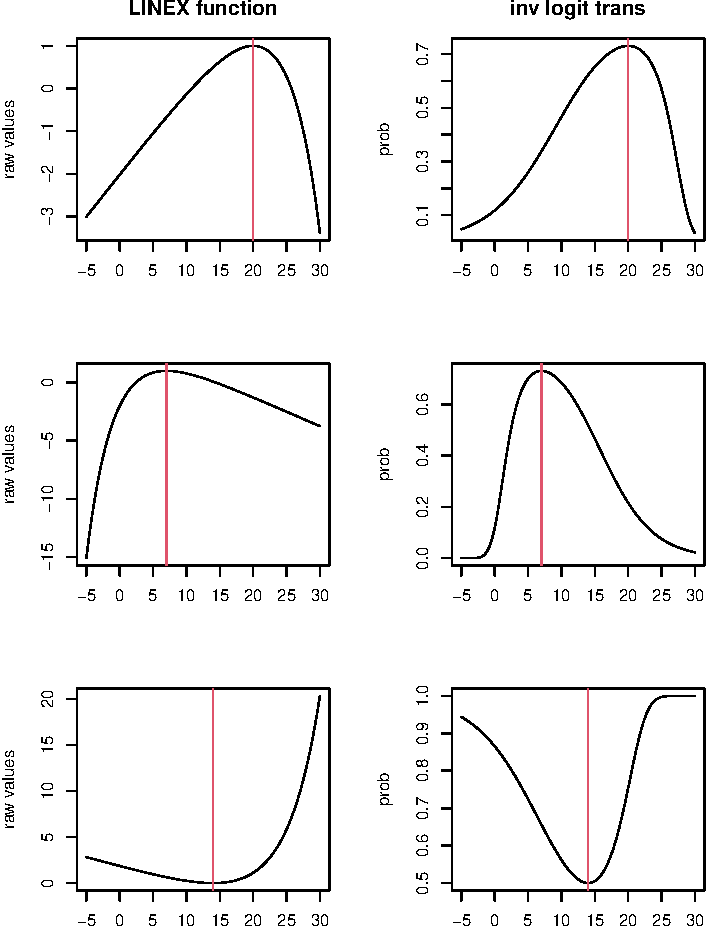
\includegraphics[keepaspectratio]{linexTPC_main_files/figure-pdf/fig-LINEX-1.pdf}}

}

\caption{\label{fig-LINEX}Examples of shapes that can be generated by
the LINEX TPC, together with a vertical line indicating the location of
the optimum. In each case, the left panel shows the shape of the
non-linear predictor and the right panel shows the inverse logit
transformed predictor that gives the probability of success. TOP:
Left-skewed, \(T_{\mathrm{opt}}=20\), \(a = 0.2\), \(c=2\). MIDDLE:
Right-skewed, \(T_{\mathrm{opt}}=7\), \(a = -0.25\), \(c=2\). BOTTOM:
concave-up, \(T_{\mathrm{opt}}=14\), \(a = 0.2\), \(c=-1\).}

\end{figure}%

We can simulate data from this model to use for testing in a
straightforward manner. We define the inverse logit transform of the
LINEX function as the probability, \(p\), for the target binomial
distribution. We first choose parameters for the LINEX function and the
number of trials in an experiment (e.g., the number of eggs). We then
draw the number of ``successes'' (eggs that hatch) using the
\texttt{rbinom} function in R with the \(p\) set as the value of \(p\)
at the temperature setting, and repeat this across a set number of
replicates (Fig~\ref{fig-simdat}). We will use these simulated data to
test the inference functions in the next section.

\begin{figure}

\centering{

\pandocbounded{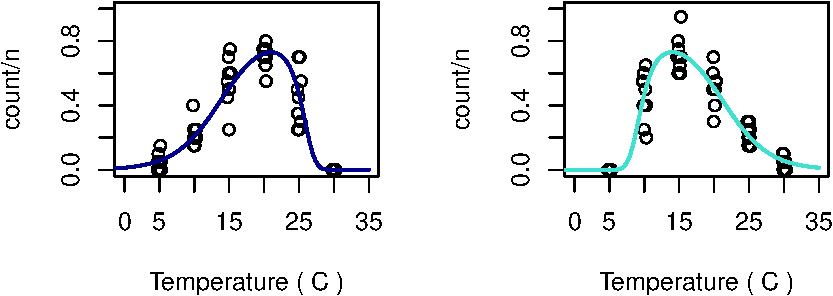
\includegraphics[keepaspectratio]{linexTPC_main_files/figure-pdf/fig-simdat-1.pdf}}

}

\caption{\label{fig-simdat}Visualization of simulated data from the
LINEX TPC model, together with inverse transform of the assumed
functional response (blue lines). Points correspond to 10 virtual
replicates, each consisting of \(n=20\) `trials' with the proportion of
successes plotted (counts/\(n\)) at each temperature. Temperature values
are jittered slightly for visualization purposes. LEFT: Left-skewed
simulation, dark blue line, \(T_{\mathrm{opt}}=21\), \(a = 0.3\),
\(c=2\). RIGHT: Right-skewed simulation, light blue line,
\(T_{\mathrm{opt}}=14\), \(a = -0.3\), \(c=2\)}

\end{figure}%

\subsection{\texorpdfstring{Bayesian inference for LINEX TPC using
\texttt{bayesTPC}}{Bayesian inference for LINEX TPC using bayesTPC}}\label{bayesian-inference-for-linex-tpc-using-bayestpc}

In R {[}12{]} and most other common statistical software, the sort of
extensions to GLMs used here are not easy to implement by default.
Typically a user would need to be able to manually specify the
predictor, link, and likelihood. This must then be inputted into an
appropriate optimization routine (to perform maximum likelihood
estimation of parameters), or priors could additionally be specified and
Bayesian estimation performed (e.g., via Markov-chain Monte Carlo). This
typically requires some specialist knowledge. However, the package
\texttt{bayesTPC} {[}13{]} in R allows for specification of TPCs and
model formulations in a relatively straightforward way. Thus we use this
package and its machinery to build a straightforward example pipeline.

Building a model in \texttt{bayesTPC} requires three steps:

\begin{enumerate}
\def\labelenumi{\arabic{enumi})}
\tightlist
\item
  defining a named TPC with corresponding formula (as an R
  ``expression'')
\item
  defining priors for all parameters that will be fitted as a vector
  with named elements
\item
  building the model using the appropriate model specification function
  -- here \texttt{specify\_binomial\_model} which assumes the
  appropriate logit link function and binomial likelihood.
\end{enumerate}

These functions build the model in the BUGS language. This resulting
model can be examined here:

\begin{verbatim}
{
    for (i in 1:N){
        logit(m[i]) <- ( -exp(-a * (Topt - Temp[i])) + a * (Temp[i] - Topt) + cc )
        Trait[i] ~ dbinom(m[i], n[i])
    }
    cc ~ dexp(0.1)
    a ~ dnorm(0, 1)
    Topt ~ dnorm(25, 1/1000)
}
\end{verbatim}

Notice that the TPC expression is defined in terms of the temperature,
which is notated as \texttt{Temp}. This is required by \texttt{bayesTPC}
to ensure that all follow-on functions work properly. Parameters can
otherwise be defined as the user prefers, although it is recommended
that parameters not share names with functions or variables that are
used elsewhere in R (for example \texttt{c} which is the concatenate
function in R, or \texttt{T} and \texttt{F} which correspond to
\texttt{TRUE} and \texttt{FALSE}).

\section{Results}\label{results}

\subsection{Performance on simulated
data}\label{performance-on-simulated-data}

The \texttt{bayesTPC} package requires that data be formatted as a list
with elements called ``Trait'' (the response being modeled) and ``Temp''
(the corresponding temperature at which the trait is measured.
Additionally, for fitting binomial models, as we are doing here, the
data list should include ``n'', the number of trials of which the
``Trait'' is the number of successes in that trial.

Once the data have been formatted and our bespoke LINEX TPC model
defined, we use the built in function \texttt{b\_TPC} to fit the model.
There are various options that can be included. Here we specify a
sampler type ``AF\_slice'' (that works well for posteriors that may have
high correlation, as TPCs often do), as well as a burn in length and
number of total iterations of the MCMC to keep (for more details about
possibilities see {[}13{]}). We also give an example of specifying a
starting value for the sampler. Although this is not strictly necessary,
it can speed up convergence.

The \texttt{bayesTPC} package includes a variety of visualization tools
that utilize \texttt{coda} {[}14{]} and similar packages to allow
checking of MCMC chain convergence, prior-posterior overlap, and
marginal and joint posterior distributions of parameters (see
Section~\ref{sec-diagL} for diagnostic plots for the model fits for the
left-skewed data). It also provides summaries of model fits, and maximum
\emph{a posteriori} (MAP) estimates of parameters. For our purposes
here, the most interesting output is the estimated median posterior TPC
and the 95\% highest posterior density (HPD) interval of this median
across temperatures (Fig~\ref{fig-simdatFits}). In the simulated data
set, we have a sufficient amount of data across a reasonably fine grid
of temperature settings. This allows the algorithm to reconstruct the
curve and parameters well.

It is important to note that as the model is so flexible, it can miss
the mark in cases where the experimental design (i.e., temperature
settings) is less than ideal. In Fig~\ref{fig-simdatFits} (bottom two
panels) we give examples of fits obtained when data at a single
temperature (here 10\(^{\circ}\)C) are removed. For the left skewed data
(Fig~\ref{fig-simdatFits}, bottom left panel), this removes data in the
longer tail, which can result in two effects. First (as shown here) we
can get a similar fit, with slightly increased uncertainty. This data
missingness can also slow convergence and result in poor fits where the
estimated skew is backwards and the peak is close to the range of the
missing data (not shown). In contrast, when the data are missing closer
to the peak as in the right-skewed data (Fig~\ref{fig-simdatFits},
bottom right panel) the right hand tail is still captured adequately,
but the uncertainty in the location of the peak increases, which also
changes the estimate of the temperature where the drop-off occurs. These
are standard issues in estimation of parameters for non-linear functions
if insufficient predictor settings are used, as has been noted by other
authors {[}7{]}.

\begin{figure}

\centering{

\pandocbounded{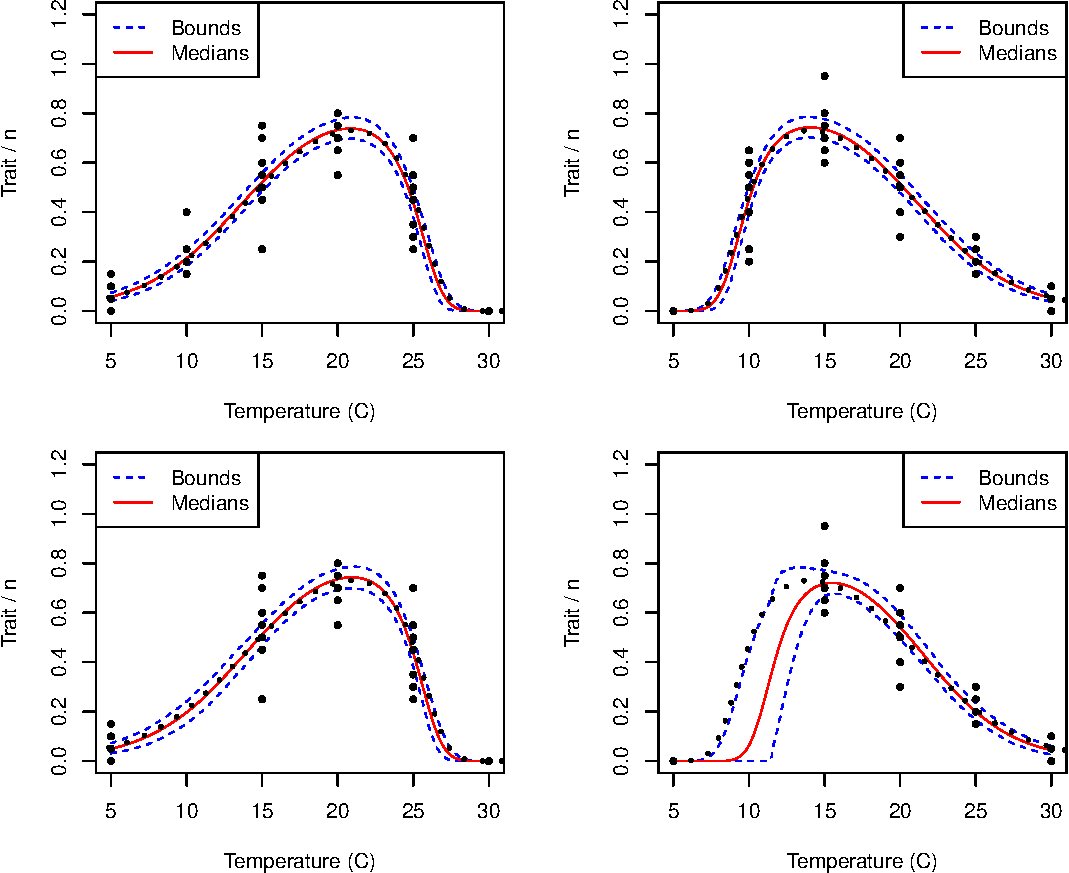
\includegraphics[keepaspectratio]{linexTPC_main_files/figure-pdf/fig-simdatFits-1.pdf}}

}

\caption{\label{fig-simdatFits}Visualization of posterior fits of the
LINEX TPC to simulated data from the LINEX TPC model from the
left-skewed (LEFT) and right-skewed (RIGHT) models show in
Fig~\ref{fig-simdat}. The TOP row shows the complete data set and the
BOTTOM row where the data at \(10^{o}\)C has been removed. The median
fit is indicated with a solid red line, the 95\% HPD interval of the TPC
as the dashed blue lines. The true line (corresponding to the model that
generated the data) is indicated with a dotted black line. Points
correspond to 10 virtual replicates, each consisting of \(n=20\)
`trials' with the proportion of successes plotted (counts/\(n\)) at each
temperature.}

\end{figure}%

\subsection{Examples using `real' arthropod TPC
data}\label{examples-using-real-arthropod-tpc-data}

Next we demonstrate the performance of the LINEX TPC on real world
experimental data, focusing on model selection. In some cases, theory
can guide the user's choice between fitting a symmetric or asymmetric
TPC. Since the LINEX function proposed here cannot capture symmetric
patterns, the user must consider assumptions and compare function choice
carefully.

Here we give examples from two similar data sets where we show how the
user could fit multiple functional forms and choose between them using
information criteria, specifically WAIC (widely-applicable information
criterion, {[}15{]}). More specifically, we explore data on the
proportion of larvae/eggs that successfully develop into adults across
temperatures for two species of mosquitoes, \emph{Aedes aegypti}
{[}16{]} and \emph{Anopheles stephensi} {[}17{]}.

\subsubsection{\texorpdfstring{Larvae to adult emergence probability for
\emph{Aedes
aegypti}}{Larvae to adult emergence probability for Aedes aegypti}}\label{larvae-to-adult-emergence-probability-for-aedes-aegypti}

Our first example is from {[}16{]}, one of the first studies to explore
the temperature dependence of emergence probability in \emph{Aedes
aegypti}. This study observed newly emerged larvae, and recorded the
proportion of these emerging as adults, at each of five fixed
temperatures. Thus, the trait aggregates survival and development across
multiple life stages (3 larval instars, and pupae), but does not include
the probability of hatching from the egg stage. We fit the LINEX TPC in
the binomial likelihood framework and a more standard quadratic GLM to
these data. We use WAIC as our metric for model selection.

As we can see in Fig~\ref{fig-HeadleeSurvFits}, the LINEX TPC is
visually a much better fit than the quadratic -- these data seem to be
fairly obviously asymmetric. The WAIC scores confirm the visual
assessment, showing that for these data, the LINEX TPC is strongly
preferred (Fig~\ref{fig-HeadleeSurvFits}).

\begin{figure}

\centering{

\pandocbounded{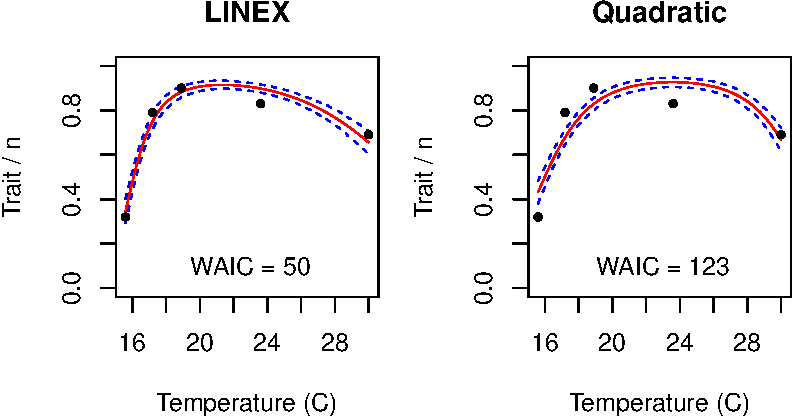
\includegraphics[keepaspectratio]{linexTPC_main_files/figure-pdf/fig-HeadleeSurvFits-1.pdf}}

}

\caption{\label{fig-HeadleeSurvFits}Visualization of posterior fits of
the LINEX TPC (left) and quadratic generalized linear model (right) to
data on probability of larvae successfully developing to the adult stage
in \emph{Aedes aegypti}across temperature (from {[}16{]}). The median
fit is indicated with a solid red line, the 95\% HPD interval of the TPC
as the dashed blue lines. WAIC for the corresponding fits are shown in
each panel}

\end{figure}%

\subsubsection{\texorpdfstring{Egg to adult emergence probability for
\emph{Anopheles
stephensi}}{Egg to adult emergence probability for Anopheles stephensi}}\label{egg-to-adult-emergence-probability-for-anopheles-stephensi}

For our second example, we examine data from {[}17{]} on the proportion
of \emph{Anopheles stephensi} eggs that successfully develop into adults
across 9 temperatures and 3 different relative humidity (RH) levels.
This trait aggregates survival and development across multiple life
stages (egg, 3 instars, and pupa) into a single metric. TPCs for this
trait are typically assumed to be symmetric (e.g., quadratic). We fit
the same two models to data at each humidity level separately, and
choose the best fitting model at each humidity level using WAIC.

\begin{figure}

\centering{

\pandocbounded{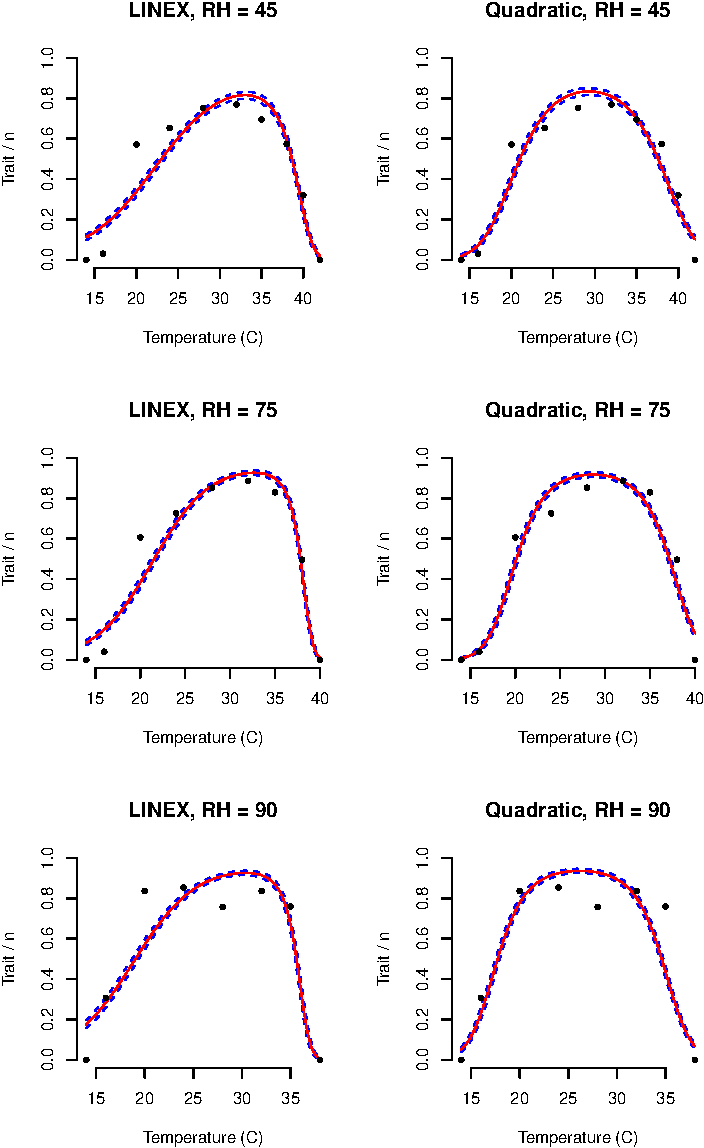
\includegraphics[keepaspectratio]{linexTPC_main_files/figure-pdf/fig-mozJuvSurvFits-1.pdf}}

}

\caption{\label{fig-mozJuvSurvFits}Visualization of posterior fits of
the LINEX TPC and quadratic generalized linear model to data on the
proportion of eggs emerging as adults across temperature for three
humidity levels (from Huxley et. al, submitted). The median fit is
indicated with a solid red line, the 95\% HPD interval of the TPC as the
dashed blue lines.}

\end{figure}%

\begin{longtable}[]{@{}rrr@{}}

\toprule\noalign{}
RH & LINEX & QUAD \\
\midrule\noalign{}
\endhead
\bottomrule\noalign{}
\endlastfoot
45 & 368.42 & 275.39 \\
75 & 285.62 & 294.16 \\
90 & 1007.58 & 642.67 \\


\caption{\label{tbl-mozJuvSurvFitsWAIC}WAIC values for the LINEX and
quadratic generalized linear model fits from
Fig~\ref{fig-mozJuvSurvFits}.}

\tabularnewline
\end{longtable}

We can see in Fig~\ref{fig-mozJuvSurvFits} that both models visually
have reasonable fits at each humidity level, although the relatively
flat emergence probability across a wide temperature range seen at 90\%
RH (bottom two rows) is not particularly well captured by either model.
Model selection via WAIC prefers the symmetric quadratic function at
most RH (including levels not shown here), but at 75\% RH the LINEX is
favored (Table~\ref{tbl-mozJuvSurvFitsWAIC}).

\section{Discussion}\label{discussion}

In this paper we introduce the use of the LINEX function, a fairly
simple non-linear function that can serve as an asymmetric TPC in a
GLM-style modeling approach. This approach can be used model bounded
data that are not well captured by a more classic piecewise continuous
bounded TPC with normal (or approximately normal) noise. We showed how
to implement analyses using the \texttt{bayesTPC} package to perform
inference in a Bayesian context, exploring both the performance on
simulated data (where parameters are known) and experimental data, where
parameters are unknown.

Often the assumed shape of a TPC reflects assumptions about the traits.
For example, compound traits, such as the probability of emergence of an
adult mosquito (which integrates over multiple life stages), are
frequently assumed to have symmetric TPCs. However, the choice of
functions for traits are not often obvious, for example, in situations
where secondary stressors may impact the trait. Thus, a practitioner
usually will need to choose between functional forms when fitting
models.

There are a wide variety of functions that have been proposed as TPCs in
thermal ecology. These functions allow users to assume a wide variety of
shapes while assuming different levels of ``mechanism'' that cause the
shape. TPC functions also vary in their flexibility. The Briere function
{[}18{]} is fairly strict, with a shape that is always left skewed (long
left-hand tail), a sharp drop off, and an assumption that minimum
performance must occur at temperatures above 0\(^\circ\)C. In contrast,
the new flexTPC {[}19{]} enables symmetric or non-symmetric shapes,
left- or right-skew, and minimum temperatures of any value. The
trade-off is an increase in the number of parameters needed to capture
the possible shapes.

A unifying feature of these TPCs that they are explicitly bounded from
below, that is the functions are \(\geq 0\). This boundedness is
important for the vast majority of TPC applications, as the performance
traits being modeled are also typically strictly \(\geq 0\). However,
this makes established TPCs inappropriate for including within a
GLM-type analysis with canonical link functions. Although it is strictly
possible to include the more traditional (typically piece-wise
continuous) TPCs in a GLM analysis using a unit link, this can create
other problems. For example, neither the Poisson distribution nor the
binomial distribution is well defined for a mean with value exactly
zero. The canonical link functions explicitly force an asymptote
\emph{towards} zero to avoid this occurring. If one is instead
truncating a function (e.g., a Briere) at particular values, this causes
instabilities in estimation under this framework. One could instead use
a small non-zero value outside of the minimum and maximum limits of the
TPC. However, doing so is equivalent to assuming a minimum rate (for
Poisson) or probability (for a binomial) that is constant across all
other values. This is both a biologically poor assumption, and one that
can bias estimation of the TPC and predictions from the model.

The LINEX TPC, together with a simple quadratic (to capture symmetric
responses), are able to represent a wide range of shapes that are
appropriate to use within the logistic model framework because they have
infinite support -- that is they can produce responses from \(-\infty\)
to \(\infty\). Further, because of this property, they are also
appropriate to model other sorts of data within the GLM-flavor
framework. For example, count data (such as may be recorded for
fecundity) could be modeled with the LINEX TPC and the log-link to
either a Poisson or negative-binomial likelihood. Thus, this relatively
simple three-parameter function can be used for a wide variety of
thermal trait (or other) data.

Although the model is fairly simple, due to the non-linearity in the
parameters, the choice of priors for Bayesian inference can still be a
bit of an art. The temptation is often to choose priors that are wide
and relatively un-informative for all parameters, but this can result in
inadequate fitting and bias. For example, if one lets both \(c\) and
\(a\) have wide priors, particularly if both can be either positive or
negative, the resulting fit can be biased. The rate of convergence can
be greatly improved by instead choosing weakly informative priors for
one or both of these parameters. For instance, if we know that our peak
probability is high-ish -- above 0.3 or so -- then a prior that
constrains \(c\) to be positive improves the inference substantially.
Further, if one has biological knowledge about the likely direction of
the skew of the trait, constraining \(a\) to reflect this will also
improve inference. In the examples given in this study, we chose weakly
informative priors to substantially improve convergence. Practitioners
taking a maximum likelihood approach would likely need to constrain
optimization routines in similar ways to obtain good results.

%\clearpage
\setstretch{1}

\section*{References}\label{references}

\phantomsection\label{refs}
\begin{CSLReferences}{0}{1}
\bibitem[\citeproctext]{ref-angilletta2002evolution}
\CSLLeftMargin{1. }%
\CSLRightInline{Angilletta Jr MJ, Niewiarowski PH, Navas CA. The
evolution of thermal physiology in ectotherms. Journal of thermal
Biology. 2002;27: 249--268. }

\bibitem[\citeproctext]{ref-huey1979integrating}
\CSLLeftMargin{2. }%
\CSLRightInline{Huey RB, Stevenson R. Integrating thermal physiology and
ecology of ectotherms: A discussion of approaches. American Zoologist.
1979;19: 357--366. }

\bibitem[\citeproctext]{ref-schoolfield1981non}
\CSLLeftMargin{3. }%
\CSLRightInline{Schoolfield RM, Sharpe P, Magnuson CE. Non-linear
regression of biological temperature-dependent rate models based on
absolute reaction-rate theory. Journal of theoretical biology. 1981;88:
719--731. }

\bibitem[\citeproctext]{ref-amarasekare2012framework}
\CSLLeftMargin{4. }%
\CSLRightInline{Amarasekare P, Savage V. A framework for elucidating the
temperature dependence of fitness. The American Naturalist. 2012;179:
178--191. }

\bibitem[\citeproctext]{ref-gajewski2021predicting}
\CSLLeftMargin{5. }%
\CSLRightInline{Gajewski Z, Stevenson LA, Pike DA, Roznik EA, Alford RA,
Johnson LR. Predicting the growth of the amphibian chytrid fungus in
varying temperature environments. Ecology and Evolution. 2021;11:
17920--17931. }

\bibitem[\citeproctext]{ref-padfield2021rtpc}
\CSLLeftMargin{6. }%
\CSLRightInline{Padfield D, O'Sullivan H, Pawar S. rTPC and nls.
Multstart: A new pipeline to fit thermal performance curves in r.
Methods in Ecology and Evolution. 2021;12: 1138--1143. }

\bibitem[\citeproctext]{ref-pawar2016real}
\CSLLeftMargin{7. }%
\CSLRightInline{Pawar S, Dell AI, Savage VM, Knies JL. Real versus
artificial variation in the thermal sensitivity of biological traits.
The American Naturalist. 2016;187: E41--E52. }

\bibitem[\citeproctext]{ref-parsian2002estimation}
\CSLLeftMargin{8. }%
\CSLRightInline{Parsian A, Kirmani S. Estimation under LINEX loss
function. Handbook of applied econometrics and statistical inference.
CRC Press; 2002. pp. 75--98. }

\bibitem[\citeproctext]{ref-singh2002estimation}
\CSLLeftMargin{9. }%
\CSLRightInline{Singh U, Gupta PK, Upadhyay S. Estimation of
exponentiated weibull shape parameters under LINEX loss function.
Communications in Statistics-Simulation and Computation. 2002;31:
523--537. }

\bibitem[\citeproctext]{ref-li2007empirical}
\CSLLeftMargin{10. }%
\CSLRightInline{Li X, Shi Y, Wei J, Chai J. Empirical bayes estimators
of reliability performances using LINEX loss under progressively type-II
censored samples. Mathematics and Computers in Simulation. 2007;73:
320--326. }

\bibitem[\citeproctext]{ref-doostparast2013bayes}
\CSLLeftMargin{11. }%
\CSLRightInline{Doostparast M, Ahmadi MV, Ahmadi J. Bayes estimation
based on joint progressive type II censored data under LINEX loss
function. Communications in Statistics-Simulation and Computation.
2013;42: 1865--1886. }

\bibitem[\citeproctext]{ref-cranR}
\CSLLeftMargin{12. }%
\CSLRightInline{R Core Team. R: A language and environment for
statistical computing. Vienna, Austria: R Foundation for Statistical
Computing; 2025. Available: \url{https://www.R-project.org/}}

\bibitem[\citeproctext]{ref-sorek2025}
\CSLLeftMargin{13. }%
\CSLRightInline{Sorek S, Smith Jr. JW, Huxley PJ, Johnson LR.
`bayesTPC`: Bayesian inference for thermal performance curves in r.
Methods in Ecology and Evolution. 2025;16: 687--697.
doi:\href{https://doi.org/10.1111/2041-210X.70004}{10.1111/2041-210X.70004}}

\bibitem[\citeproctext]{ref-coda}
\CSLLeftMargin{14. }%
\CSLRightInline{Plummer M, Best N, Cowles K, Vines K. CODA: Convergence
diagnosis and output analysis for MCMC. R News. 2006;6: 7--11.
Available: \url{https://journal.r-project.org/archive/}}

\bibitem[\citeproctext]{ref-gelman2013infcrit}
\CSLLeftMargin{15. }%
\CSLRightInline{Gelman A, Hwang J, Vehtari A. Understanding predictive
information criteria for bayesian models. Statistics and Computing.
2013;24. }

\bibitem[\citeproctext]{ref-headlee1942continuation}
\CSLLeftMargin{16. }%
\CSLRightInline{Headlee TJ. A continuation of the studies of the
relative effects on insect metabolism of temperature derived from
constant and varied sources. Journal of Economic Entomology. 1942;35:
785--786. }

\bibitem[\citeproctext]{ref-huxley2025beyond}
\CSLLeftMargin{17. }%
\CSLRightInline{Huxley PJ, Brown JJ, St. Laurent B, Johnson B, Cheung
OY, Asamoah A, et al. Beyond temperature: Relative humidity
systematically shifts the temperature dependence of population growth in
a malaria vector. bioRxiv. 2025; 2025--05. }

\bibitem[\citeproctext]{ref-briere1999novel}
\CSLLeftMargin{18. }%
\CSLRightInline{Briere J-F, Pracros P, Le Roux A-Y, Pierre J-S. A novel
rate model of temperature-dependent development for arthropods.
Environmental Entomology. 1999;28: 22--29. }

\bibitem[\citeproctext]{ref-cruz2024flexible}
\CSLLeftMargin{19. }%
\CSLRightInline{Cruz-Loya M, Mordecai EA, Savage VM. A flexible model
for thermal performance curves. bioRxiv. 2024. }

\end{CSLReferences}

\clearpage

\setcounter{section}{0}
\renewcommand{\thesection}{\Alph{section}}

\setcounter{table}{0}
\renewcommand{\thetable}{A\arabic{table}}

\setcounter{figure}{0}
\renewcommand{\thefigure}{A\arabic{figure}}

\section{Appendix}\label{sec-app}

\subsection{Diagnostics and summary for fit of left-skewed simulation
example}\label{sec-diagL}

\begin{figure}

\centering{

\pandocbounded{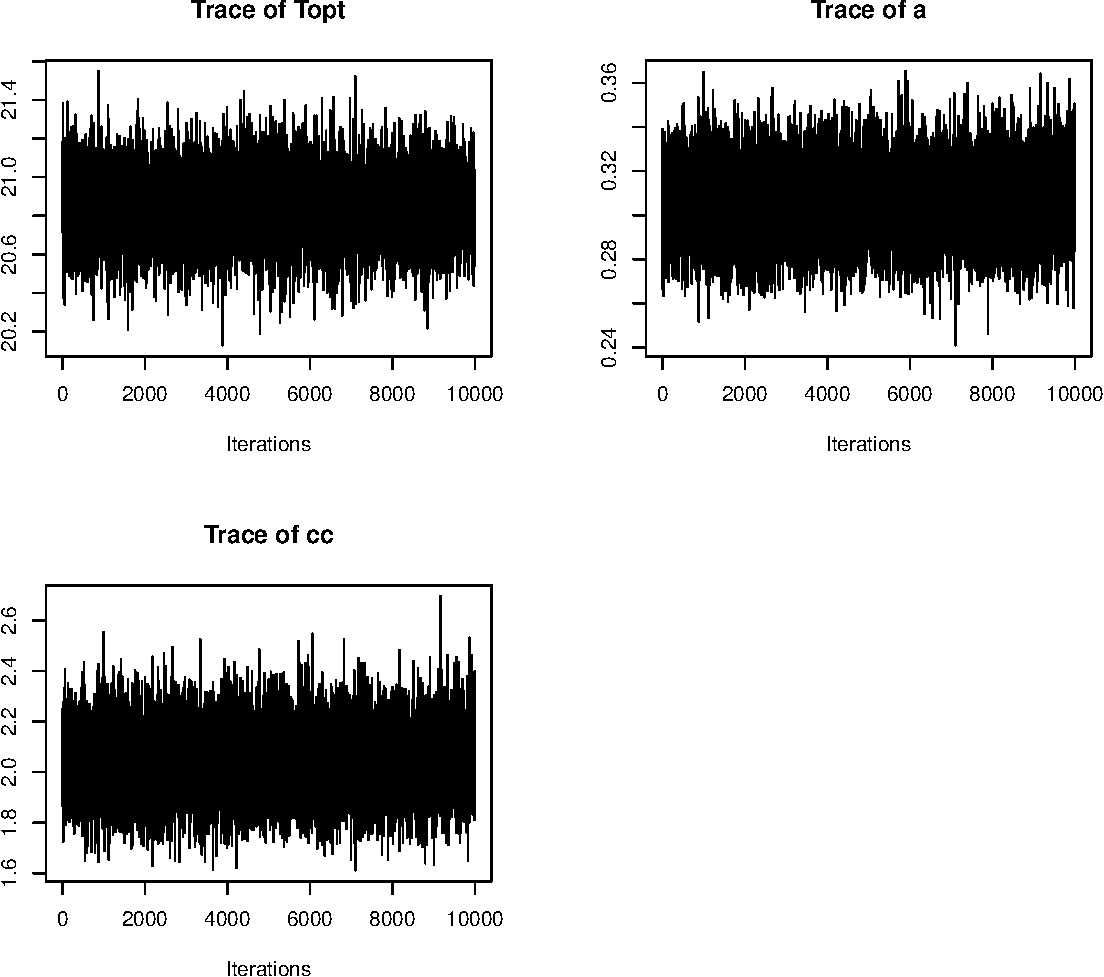
\includegraphics[keepaspectratio]{linexTPC_main_files/figure-pdf/fig-TraceLS-1.pdf}}

}

\caption{\label{fig-TraceLS}Trace plots for the LINEXP model fit to the
left skewed simulation data.}

\end{figure}%

\begin{figure}

\centering{

\pandocbounded{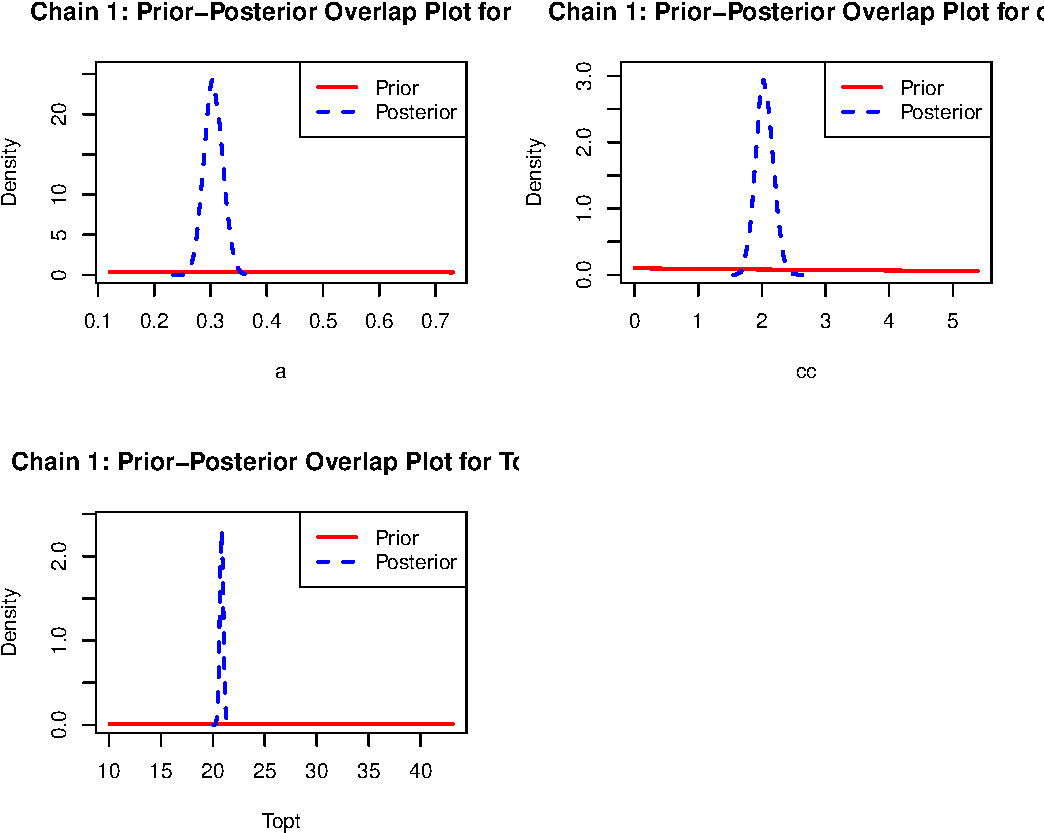
\includegraphics[keepaspectratio]{linexTPC_main_files/figure-pdf/fig-PPLS-1.pdf}}

}

\caption{\label{fig-PPLS}Prior-posterior overlap plots for the LINEXP
model fit to the left skewed simulation data.}

\end{figure}%

\begin{figure}

\centering{

\pandocbounded{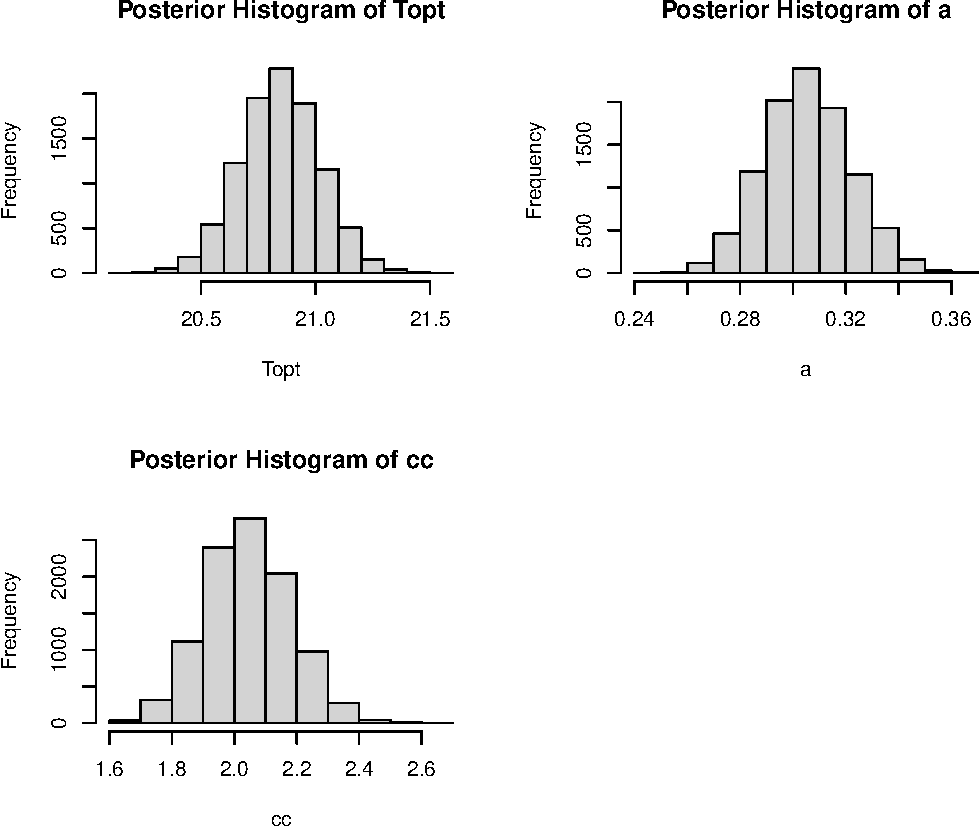
\includegraphics[keepaspectratio]{linexTPC_main_files/figure-pdf/fig-MargLS-1.pdf}}

}

\caption{\label{fig-MargLS}Histograms of the marginal posterior samples
of parameters for the LINEXP model fit to the left skewed simulation
data.}

\end{figure}%

\begin{figure}

\centering{

\pandocbounded{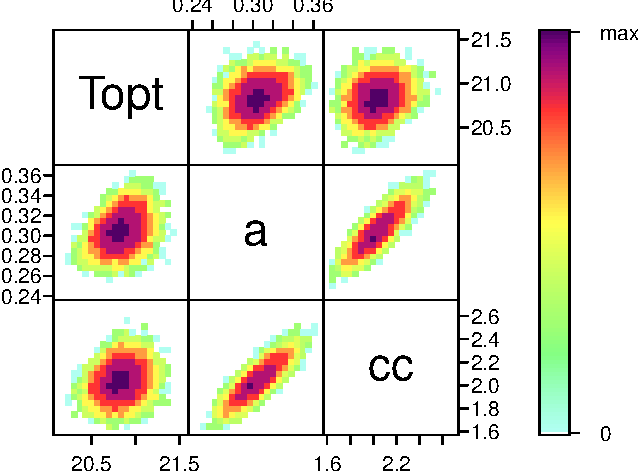
\includegraphics[keepaspectratio]{linexTPC_main_files/figure-pdf/fig-JointLS-1.pdf}}

}

\caption{\label{fig-JointLS}Pairs plot of samples from the joint
posterior of parameters for the LINEXP model fit to the left skewed
simulation data.}

\end{figure}%

\clearpage

\begin{verbatim}
bayesTPC MCMC of Type:
  LinExp_binom

Formula:
  logit(m[i]) <- ( -exp(-a * (Topt - Temp)) + a * (Temp - Topt) + cc )

Distribution:
  Trait[i] ~ dbinom(m[i], n[i])

Priors:
  cc ~ dexp(0.1) 
  a ~ dnorm(0, 1) 
  Topt ~ dnorm(25, 1/1000)

Max. A Post. Parameters: 
     Topt         a        cc  log_prob 
  20.8308    0.3059    2.0484 -110.2263 

MCMC Results:
Iterations = 1:10000
Thinning interval = 1 
Number of chains = 1 
Sample size per chain = 10000 

1. Empirical mean and standard deviation for each variable,
   plus standard error of the mean:

        Mean      SD  Naive SE Time-series SE
Topt 20.8495 0.17646 0.0017646      0.0018403
a     0.3054 0.01684 0.0001684      0.0001822
cc    2.0439 0.13906 0.0013906      0.0014876

2. Quantiles for each variable:

        2.5%     25%     50%     75%   97.5%
Topt 20.5008 20.7352 20.8486 20.9687 21.1932
a     0.2733  0.2939  0.3052  0.3168  0.3392
cc    1.7783  1.9501  2.0400  2.1365  2.3190
\end{verbatim}


\nolinenumbers


\end{document}
